\documentclass{standalone}
\usepackage{tikz}
\usetikzlibrary{patterns, positioning}


\begin{document}
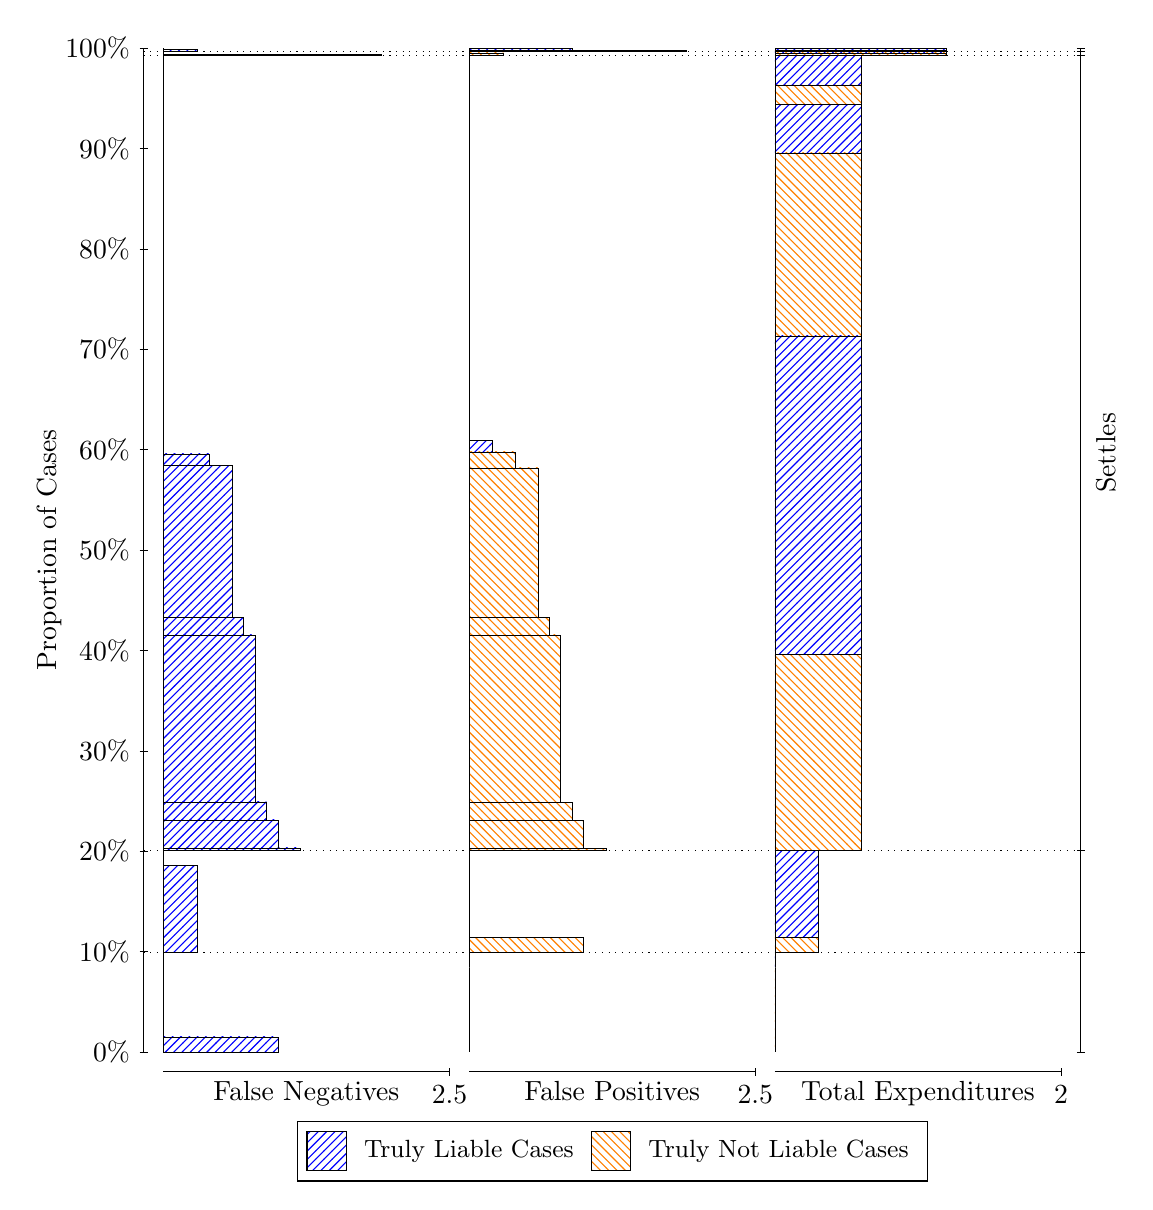
\begin{tikzpicture}
\draw[black, very thin] (1.5,1.75) -- (1.5,14.5);
\node[rotate=90, text=black, anchor=center] at (0.3, 8.125) {Proportion of Cases};
\draw[black, very thin] (1.45,1.75) -- (1.55,1.75);
\node[text=black, anchor=east] at (1.45, 1.75) {0\%};
\draw[black, very thin] (1.45,3.025) -- (1.55,3.025);
\node[text=black, anchor=east] at (1.45, 3.025) {10\%};
\draw[black, very thin] (1.45,4.3) -- (1.55,4.3);
\node[text=black, anchor=east] at (1.45, 4.3) {20\%};
\draw[black, very thin] (1.45,5.575) -- (1.55,5.575);
\node[text=black, anchor=east] at (1.45, 5.575) {30\%};
\draw[black, very thin] (1.45,6.85) -- (1.55,6.85);
\node[text=black, anchor=east] at (1.45, 6.85) {40\%};
\draw[black, very thin] (1.45,8.125) -- (1.55,8.125);
\node[text=black, anchor=east] at (1.45, 8.125) {50\%};
\draw[black, very thin] (1.45,9.4) -- (1.55,9.4);
\node[text=black, anchor=east] at (1.45, 9.4) {60\%};
\draw[black, very thin] (1.45,10.675) -- (1.55,10.675);
\node[text=black, anchor=east] at (1.45, 10.675) {70\%};
\draw[black, very thin] (1.45,11.95) -- (1.55,11.95);
\node[text=black, anchor=east] at (1.45, 11.95) {80\%};
\draw[black, very thin] (1.45,13.225) -- (1.55,13.225);
\node[text=black, anchor=east] at (1.45, 13.225) {90\%};
\draw[black, very thin] (1.45,14.5) -- (1.55,14.5);
\node[text=black, anchor=east] at (1.45, 14.5) {100\%};

\draw[black, very thin] (13.4,1.75) -- (13.4,14.5);
\draw[black, very thin] (13.35,1.75) -- (13.45,1.75);
\node[anchor=west] at (13.35, 1.75) {};
\draw[black, very thin] (13.35,3.0143) -- (13.45,3.0143);
\node[anchor=west] at (13.35, 3.0143) {};
\draw[black, very thin] (13.35,4.3118) -- (13.45,4.3118);
\node[anchor=west] at (13.35, 4.3118) {};
\draw[black, very thin] (13.35,14.404) -- (13.45,14.404);
\node[anchor=west] at (13.35, 14.404) {};
\draw[black, very thin] (13.35,14.453) -- (13.45,14.453);
\node[anchor=west] at (13.35, 14.453) {};
\draw[black, very thin] (13.35,14.5) -- (13.45,14.5);
\node[anchor=west] at (13.35, 14.5) {};

\draw[black, very thin, pattern color=blue, pattern=north east lines] (1.75,1.75) rectangle (3.2033,1.9425);
\draw[black, very thin, pattern color=orange, pattern=north west lines] (1.75,1.9425) rectangle (1.75,3.0143);
\draw[black, very thin, pattern color=blue, pattern=north east lines] (1.75,3.0143) rectangle (2.186,4.1168);
\draw[black, very thin, pattern color=orange, pattern=north west lines] (1.75,4.1168) rectangle (1.75,4.3118);
\draw[black, very thin, pattern color=blue, pattern=north east lines] (1.75,4.3118) rectangle (3.494,4.3429);
\draw[black, very thin, pattern color=blue, pattern=north east lines] (1.75,4.3429) rectangle (3.2033,4.6977);
\draw[black, very thin, pattern color=blue, pattern=north east lines] (1.75,4.6977) rectangle (3.058,4.925);
\draw[black, very thin, pattern color=blue, pattern=north east lines] (1.75,4.925) rectangle (2.9127,7.0481);
\draw[black, very thin, pattern color=blue, pattern=north east lines] (1.75,7.0481) rectangle (2.7673,7.2739);
\draw[black, very thin, pattern color=blue, pattern=north east lines] (1.75,7.2739) rectangle (2.622,9.1981);
\draw[black, very thin, pattern color=blue, pattern=north east lines] (1.75,9.1981) rectangle (2.3313,9.3448);
\draw[black, very thin, pattern color=orange, pattern=north west lines] (1.75,9.3448) rectangle (1.75,14.404);
\draw[black, very thin, pattern color=blue, pattern=north east lines] (1.75,14.404) rectangle (4.5113,14.42);
\draw[black, very thin, pattern color=orange, pattern=north west lines] (1.75,14.42) rectangle (1.75,14.453);
\draw[black, very thin, pattern color=blue, pattern=north east lines] (1.75,14.453) rectangle (2.186,14.484);
\draw[black, very thin, pattern color=orange, pattern=north west lines] (1.75,14.484) rectangle (1.75,14.5);
\draw[black, very thin, pattern color=orange, pattern=north west lines] (5.6333,1.75) rectangle (5.6333,2.8218);
\draw[black, very thin, pattern color=blue, pattern=north east lines] (5.6333,2.8218) rectangle (5.6333,3.0143);
\draw[black, very thin, pattern color=orange, pattern=north west lines] (5.6333,3.0143) rectangle (7.0867,3.2093);
\draw[black, very thin, pattern color=blue, pattern=north east lines] (5.6333,3.2093) rectangle (5.6333,4.3118);
\draw[black, very thin, pattern color=orange, pattern=north west lines] (5.6333,4.3118) rectangle (7.3773,4.3351);
\draw[black, very thin, pattern color=orange, pattern=north west lines] (5.6333,4.3351) rectangle (7.0867,4.6932);
\draw[black, very thin, pattern color=orange, pattern=north west lines] (5.6333,4.6932) rectangle (6.9413,4.9205);
\draw[black, very thin, pattern color=orange, pattern=north west lines] (5.6333,4.9205) rectangle (6.796,7.0459);
\draw[black, very thin, pattern color=orange, pattern=north west lines] (5.6333,7.0459) rectangle (6.6507,7.2717);
\draw[black, very thin, pattern color=orange, pattern=north west lines] (5.6333,7.2717) rectangle (6.5053,9.1679);
\draw[black, very thin, pattern color=orange, pattern=north west lines] (5.6333,9.1679) rectangle (6.2147,9.3711);
\draw[black, very thin, pattern color=blue, pattern=north east lines] (5.6333,9.3711) rectangle (5.924,9.5177);
\draw[black, very thin, pattern color=blue, pattern=north east lines] (5.6333,9.5177) rectangle (5.6333,14.404);
\draw[black, very thin, pattern color=orange, pattern=north west lines] (5.6333,14.404) rectangle (6.0693,14.437);
\draw[black, very thin, pattern color=blue, pattern=north east lines] (5.6333,14.437) rectangle (5.6333,14.453);
\draw[black, very thin, pattern color=orange, pattern=north west lines] (5.6333,14.453) rectangle (8.3947,14.469);
\draw[black, very thin, pattern color=blue, pattern=north east lines] (5.6333,14.469) rectangle (6.9413,14.5);
\draw[black, very thin, pattern color=orange, pattern=north west lines] (9.5167,1.75) rectangle (9.5167,2.8218);
\draw[black, very thin, pattern color=blue, pattern=north east lines] (9.5167,2.8218) rectangle (9.5167,3.0143);
\draw[black, very thin, pattern color=orange, pattern=north west lines] (9.5167,3.0143) rectangle (10.062,3.2093);
\draw[black, very thin, pattern color=blue, pattern=north east lines] (9.5167,3.2093) rectangle (10.062,4.3118);
\draw[black, very thin, pattern color=orange, pattern=north west lines] (9.5167,4.3118) rectangle (10.607,6.7953);
\draw[black, very thin, pattern color=blue, pattern=north east lines] (9.5167,6.7953) rectangle (10.607,10.843);
\draw[black, very thin, pattern color=orange, pattern=north west lines] (9.5167,10.843) rectangle (10.607,13.168);
\draw[black, very thin, pattern color=blue, pattern=north east lines] (9.5167,13.168) rectangle (10.607,13.781);
\draw[black, very thin, pattern color=orange, pattern=north west lines] (9.5167,13.781) rectangle (10.607,14.032);
\draw[black, very thin, pattern color=blue, pattern=north east lines] (9.5167,14.032) rectangle (10.607,14.404);
\draw[black, very thin, pattern color=orange, pattern=north west lines] (9.5167,14.404) rectangle (11.697,14.437);
\draw[black, very thin, pattern color=blue, pattern=north east lines] (9.5167,14.437) rectangle (11.697,14.453);
\draw[black, very thin, pattern color=orange, pattern=north west lines] (9.5167,14.453) rectangle (11.697,14.469);
\draw[black, very thin, pattern color=blue, pattern=north east lines] (9.5167,14.469) rectangle (11.697,14.5);
\draw[black, dotted] (1.5,3.0143) -- (13.4,3.0143);
\draw[black, dotted] (1.5,4.3118) -- (13.4,4.3118);
\draw[black, dotted] (1.5,14.404) -- (13.4,14.404);
\draw[black, dotted] (1.5,14.453) -- (13.4,14.453);
\draw[black, very thin] (1.75,1.5) -- (5.3833,1.5);
\node[text=black, anchor=north] at (3.5667, 1.5) {False Negatives};
\draw[black, very thin] (5.3833,1.45) -- (5.3833,1.55);
\node[text=black, anchor=north] at (5.3833, 1.45) {2.5};

\draw[black, very thin] (5.6333,1.5) -- (9.2667,1.5);
\node[text=black, anchor=north] at (7.45, 1.5) {False Positives};
\draw[black, very thin] (9.2667,1.45) -- (9.2667,1.55);
\node[text=black, anchor=north] at (9.2667, 1.45) {2.5};

\draw[black, very thin] (9.5167,1.5) -- (13.15,1.5);
\node[text=black, anchor=north] at (11.333, 1.5) {Total Expenditures};
\draw[black, very thin] (13.15,1.45) -- (13.15,1.55);
\node[text=black, anchor=north] at (13.15, 1.45) {2};



\node[text=black, centered, rotate=90] at (13.72, 9.3579) {Settles};



\draw (7.449999999999999,1.5) node[draw=none] (baseCoordinate) {};
\begin{scope}[align=center]
        \matrix[scale=0.5, draw=black, below=0.5cm of baseCoordinate, nodes={draw}, column sep=0.1cm]{
            \node[rectangle, draw, minimum width=0.5cm, minimum height=0.5cm, pattern color=blue, pattern=north east lines] {}; &
            \node[draw=none, font=\small, text=black] (B) {Truly Liable Cases}; &
            \node[rectangle, draw, minimum width=0.5cm, minimum height=0.5cm, pattern color=orange, pattern=north west lines] {}; &
            \node[draw=none, font=\small, text=black] (B) {Truly Not Liable Cases}; \\
            };
\end{scope}

\end{tikzpicture}
\end{document}